\documentclass[12pt]{article}
\usepackage[12pt]{moresize}
\usepackage[margin=1in]{geometry}

\usepackage{amsmath}
\usepackage{amssymb}

\usepackage{graphicx}
\usepackage{subcaption}

\usepackage{multirow} %Combining rows in tables
\usepackage{diagbox}  %Table box split in twain

\usepackage{algorithm}
\usepackage{algpseudocode}
\usepackage{alltt}

\usepackage{multicol}

\usepackage{amssymb} %\checkmark symbol

%\usepackage{hyperref}
%\usepackage[latin1]{inputenc}
%\usepackage{listings}
%\usepackage{scrextend}
%\usepackage{changepage} %Adjustwidth

 

\title{ComS 474\\Homework 4}
\author{Sean Gordon}
\date{Oct 11, 2020}

\begin{document}
\maketitle



\noindent 1) $
\begin{pmatrix}
w1\\ w2\\ w3
\end{pmatrix}
= \lambda_1 *
\begin{pmatrix}
a_1\\ b_1\\ c_1
\end{pmatrix}
- \lambda_3 *
\begin{pmatrix}
a_3\\ b_3\\ c_3
\end{pmatrix}
= 4.5 * (1) *
\begin{pmatrix}
.5\\ .25\\ .125
\end{pmatrix}
+ 1.5 * (-1) *
\begin{pmatrix}
.3\\ .75\\ .325
\end{pmatrix}
=
\begin{pmatrix}
1.8\\ 0\\ .075
\end{pmatrix}$\\\\

Prediction = $(1, 1, 0)*
\begin{pmatrix}
1.8\\ 0\\ .075
\end{pmatrix}
+ 1 = 2.8 > 0$, thus the predicted class is 1.\\



\noindent \hrulefill \\



\noindent 2) As the gutters span from $wx+w_b-1$ to $wx+w_b+1$, the size of the margin is {\Large$\frac{2}{||w||}$}, and the size of each gutter is 1/2 that $\Rightarrow$ {\Large$\frac{1}{||w||}$} = {\Large$\frac{1}{\sqrt{w_1^2+w_2^2}}$} = {\Large$\frac{1}{\sqrt{1.8^2+.075^2}}$} = {\Large$\frac{1}{1.802}$} = 0.555.\\\\
However, the professor has specified that $d_1$ and $d_2$ are both 1, so the equations for both gutters are: $wx+w_b\pm1=0$ $\Rightarrow$\\\\[.4em]$
\begin{pmatrix}
1.8\\ 0\\ .075
\end{pmatrix}
*x + 1 = -1$\\[.4em]
\indent \indent \indent and\\[.4em]$
\begin{pmatrix}
1.8\\ 0\\ .075
\end{pmatrix}
*x + 1 = 1 $\\




\noindent \hrulefill \\\pagebreak



\noindent 3) A point is inside the margin when $|wx+w_b| < 2d$ = $|wx+1| < 1.11$\\[.4em]
\indent (1) $|(0.5, 0.25, 0.125)*
\begin{pmatrix}
1.8\\ 0\\ .075
\end{pmatrix}
 + 1|= 1.909 > 1.11$, so this sample is outside the margin.\\[.4em]

\indent (2) $|(0.4, 0.15, 0.225)*
\begin{pmatrix}
1.8\\ 0\\ .075
\end{pmatrix}
 + 1|= 1.737 > 1.11$, so this sample is outside the margin.\\[.4em]

\indent (3) $|(0.3, 0.75, 0.325)*
\begin{pmatrix}
1.8\\ 0\\ .075
\end{pmatrix}
 + 1|= 1.564 > 1.11$, so this sample is outside the margin.\\[.4em]

\indent (4) $|(0.2, 0.65, 0.425)*
\begin{pmatrix}
1.8\\ 0\\ .075
\end{pmatrix}
 + 1|= 1.392 > 1.11$, so this sample is outside the margin.\\



\noindent \hrulefill \\



\noindent 4) \\
\indent (1) If $y_i = 1$ and $w^Tx_i+w_b \le -1$, $y_i(w^Tx_i+w_b) \le -1$, disproving the condition.\\\\
\indent (2) This condition holds for $y_i = 1$ and $w^Tx_i+w_b \le -1$ and for $y_i = -1$ and $w^Tx_i+w_b \le 1$. \\
\indent \indent Both of these sets of values when input into $y_i(w^Tx_i+w_b) \le -1$\\\\
\indent (3) If $y_i = 1$ and $w^Tx_i+w_b \le -1$, $y_i(w^Tx_i+w_b) \le -1$, disproving the condition.\\\\
\indent (4) This condition holds for $y_i = 1$ and $w^Tx_i+w_b \le -1$ and for $y_i = -1$ and $w^Tx_i+w_b \le 1$. \\
\indent \indent Both of these sets of values when input into $y_i(w^Tx_i+w_b) \le 1$\\\\
\indent (5) If $y_i = 1$ and $w^Tx_i+w_b \le -1$, $y_i(w^Tx_i+w_b) \le -1$, disproving the condition.\\\\
\indent (6) This condition holds for $y_i = 1$ and $w^Tx_i+w_b \le -1$ and for $y_i = -1$ and $w^Tx_i+w_b \le 1$. \\
\indent \indent Both of these sets of values when input into $y_i(w^Tx_i+w_b) \le 0$\\\\


%\begin{figure}[htbp]
%\centerline{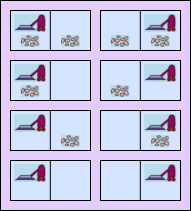
\includegraphics{Pics/ComS472_410.png}}
%\caption{Belief states recheable from initial 8 belief states.}
%\label{Belief states recheable from initial 8 belief states.}
%\end{figure}

\end{document}

















